\chapter{Attaques physiques sur EC}
\section{Présentation}
Introduction : cf fractures cryptographiques, utilisation du sons pour clavier, émanations électromagnétiques pour écran d'ordinateur, expliquer que dans le domaine militaire ces techniques sont étudiées, connues depuis bien plus longtemps que dans le domaine public.

Deux grands modèles d'attaques : modèles en boîte noire et modèle en boîte blanche (plus réaliste). 

Taxonomie des attaques par canaux auxiliaires : passives, actives (invasives et non invasives). Faire un schéma.

Parmi les attaques passives, on distingue :
\begin{itemize}[label=$\bullet$]
    \item Attaque simple / avancée. Simple SCA includes all Vertical or Horizontal SCA where the adversary makes observations on a single input. \footnote{En théorie, les attaques simples SCA peuvent être menées avec une seule observation. En pratique, cependant, il est souvent nécessaire d'utiliser plusieurs observations de la même variable $x$ afin de réduire le bruit.} Les attaques sont qualifiées d'avancées lorsque les observations impliquent plusieurs entrées. \footnote{Ainsi une attaque horizontale est nécessairement une attaque simple.}
    
    \item Attaque horizontale / verticale. Horizontale : plusieurs réalisations de variables aléatoires prises dans une seule trace. Lorsque l'attaque utilise des techniques horizontales et verticales, on la qualifie de rectangle.
    
    \item Univariée / multivariée. Lorsque les différents instants $t$ des traces sont considérées séparément, de manière indépendante ou pas. 
\end{itemize}
Une trace est un vecteur de réel, noté $l_i \in \R{}^t$. Une trace est une réalisation d'un vecteur aléatoire. Même avec les mêmes données et opérations, on obtiendra jamais la même trace. 

C'est un véritable jeu du chat et la souris, attaques et contre-mesures.

Pour les différentes classes d'attaques physiques que nous allons voir, on peut identifier deux types de contre-mesures : les \emph{protections matérielles} et les \emph{contre-mesures logicielles}. La première cherche à modifier la conception des appareils cryptographiques afin  de diminuer les fuites d'informations à travers les canaux auxiliaires. La seconde vise à construire différentes méthodes implémentant la même opération de telle façon que les informations obtenues des canaux auxiliaires soient inutiles. 

La méthodologie générale (logiciel) visant à empêcher des fuites via des canaux auxiliaires, se fait en deux étapes. La première étape consiste à rendre les attaques simples (SSCA) impossible puis dans un second temps on s'occupe des attaques différentielles (DSCA).

\section{Attaques temporelles}
Cette classe d'attaque tire profit des variations temporelles dans le calcul des opérations du corps fini. 

Il faut que toutes les opérations dans le corps fini soient implémentées en temps constant (\emph{constant time of field operations}). Par exemple il faut faire attention à la soustraction conditionnelle dans la réduction de Montgomery. Ou encore à l'addition modulaire qui implique une soustraction conditionnelle. 

\section{Attaques simples par canaux auxiliaires}
\subsection{Présentation}
Un algorithme de multiplication scalaire consiste dans un premier temps à coder le scalaire en binaire ou bien en représentation signée avec ou sans la propriété de non adjacence par exemple. Puis l'algorithme parcourt ce codage en partant du poids fort ou du poids faibles et effectue des opérations (un doublement suivit ou pas d'une addition) à chaque itération. Finalement, un algorithme de multiplication scalaire ne fait rien d'autre que de définir une séquence d'addition et de doublement permettant d'atteindre le point $[k]P$ désiré.

Cependant pour les algorithmes basiques cette séquence caractérise complètement le scalaire $k$. En d'autres termes, à chaque séquence d'addition et doublement correspond un unique scalaire. Entendons-nous bien, pour chaque valeur de $k$, il existe une infinité de séquences d'opérations \footnote{On peut toujours ajouter des opérations factices.} aboutissant à $[k]P$. Mais pour les algorithmes basiques, retrouver cette séquence revient à retrouver $k$. 

Les attaques simples par canaux auxiliaires partent du principe que la consommation électrique \footnote{Ou n'importe quelle autre canaux auxiliaires.} dépend des opérations effectuées. En particulier, si le pattern ou la \og signature \fg{} associé à l'addition et aux doublements est différentes, on peut espérer, à l'aide d'une trace, d'être en mesure de distinguer les additions des doublements.

Deux types de contre-mesures peuvent être envisagées. On peut chercher à casser le lien existant entre le scalaire $k$ et la séquence calculée. Faire en sorte que l'algorithme de SM induise une séquence d'addition et de doublement indépendante du scalaire $k$. La retrouver n'apporterait plus rien à l'attaquant. Ou bien, on peut agir sur la couche inférieure. Le principe est de modifier les formules d'addition et de doublement afin de les rendre indistinguable par analyse de leur consommation électrique. 


\subsection{Contre-mesures}
\begin{description}
    \item[Algorithme de multiplication scalaire régulier] \hfill \\ \'A chaque itération de l'algorithme, la même suite d'opération est effectuée. La séquence d'addition et de doublement définie par l'algorithme de SM est indépendante de la valeur secrète. Il n'y a plus de bijection entre la séquence d'addition et de doublement et la valeur secrète. La séquence associée à un algorithme régulier est constante, toujours la même et ceux quelque soit le scalaire. Retrouver cette séquence via une SPA n'apporte ainsi aucune information à l'attaquant.
        \begin{itemize}[label=--]
            \item Via l'insertion d'opérations factices : double-and-add always (Coron 99) qui est un double-and-add auquel on a enlevé les branchements conditionnels \cite{coron1999resistance} et qui effectue une addition même si le bit vaut 0. En plus d'être coûteuse, cette solution est sensible aux attaques par injections de fautes \footnote{C Safe Error attacks.}.
            \item Algorithme de type Ladder. Il existe l'échelle de Montgomery (87) qui peut-être vue comme un add-and-double always mais sans opérations factices cette fois. Il existe sa variante en right-to-left appelée Joye Ladder. Il existe la version coZ de ces algorithmes. Il existe aussi une variante pour les courbes elliptiques sur corps binaires \cite{lopez1999fast}.
            \item Recodage régulier. Par exemple il peut s'agir de recoder le scalaire de tel sorte que tous les bits soient non nuls. 
        \end{itemize}
        \begin{figure}[ht]
        \centering
        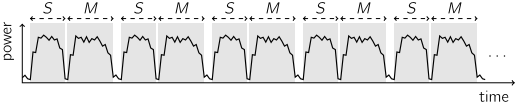
\includegraphics[scale=0.5]{images/SSCA_regular.png}
        \caption{Trace d'un algorithme régulier}
        \label{fig:SSCA_regular}
        \end{figure}
    
    \item[Principes d'atomicité] \hfill \\
    \begin{enumerate}
        \item Formules unifiées : réécrire les formules d'addition et de doublement de telles sortes qu'elles requièrent les mêmes opérations dans le corps de base. Pour certaines formes de courbes, les formules sont naturellement unifiées (voires complètes) : elles s'appliquent que les points en entrées soient identiques ou non. L'attaquant ne pourra plus distinguer quelle opération est effectuée puisque leur consommation électrique sera la même. Il obtiendra une séquence constante d'addition. 
        
        Il est possible de réécrire l'expression du coefficient directeur \footnote{Slope, pente.} $\lambda$ afin qu'il soit valable pour l'addition et le doublement. Les formes Hessiennes ont des formules unifiées assez efficace. Le doublement peut en fait s'écrire comme une addition $[2](X : Y : Z) = (Z : X : Y) + (Y : Z : X)$. Les formes d'Edwards possèdent une arithmétique efficace et intrinsèquement unifiées voire même complète en fonction du paramètre $d$ choisi. 
        
        Notez que cette contre-mesure présente quelques défauts qu'il est important de mentionner :
        \begin{itemize}[label=--]
            \item L'emploie de formules unifiées ne permet pas toujours d'empêcher une SSCA. En effet si l'attaquant est capable d'identifier le passage d'une itération à l'autre, alors il pourra retrouver la séquence d'opération calculée \footnote{En supposant qu'il n'a pas implémenté un algorithme régulier.}. Un bloc constitué de deux opérations représentera un bit égal à $1$. C'est la raison pour laquelle, il est souvent conseillé d'associer des formules unifiées avec un double-and-add atomic. Dans ce cas à chaque itération, une seule opération est effectuée, la consommation électrique de chaque opération se trouve ainsi espacée de manière régulière. 
            \item En supposant que la longueur du scalaire est connue, cette contre-mesure laisse fuir le poids de Hamming de la valeur secrète. En effet le nombre de doublement correspond à la longueur du scalaire et le nombre réel d'addition correspond au poids de Hamming du scalaire. Laisser fuir cette information n'est pas très dangereux et il est possible de masquer le scalaire par des techniques de randomnisation.
        \end{itemize}
        
        \item Atomicité au niveau du corps de base \footnote{Pour ECC mais pas pour RSA.}. L'idée consiste à décomposer l'addition et le doublement en une séquence fixe d'opération dans le corps de base. Cette séquence est appelée un \emph{bloc atomique}. Par exemple une addition peut se calculer par la répétition de $161$ blocs atomiques tandis que le doublement se calcule par une succession de $10$ blocs atomiques. 
        
        Cette contre-mesure présente toutefois deux inconvénients. Le premier est qu'elle remplace les carrés par des multiplications plus coûteuses. Le second est qu'elle introduit des additions, soustractions factices.
        \begin{itemize}[label=--]
            \item Original ECC pattern (Chevallier et al., 03), \cite{chevallier2004low}. 
            \item Longa ECC pattern (Longa, 07), \cite{longa2007accelerating}.
            \item Improved ECC pattern (Girault et Verneuil, 10), \cite{giraud2010atomicity}.
            \item \cite{rondepierre2014revisiting}
        \end{itemize}    
    \end{enumerate}
\end{description}

Il existe des attaques horizontales contres le principe d'atomicité (formules unifiées ou atomicité dans le corps de base) : Big Mac, Big Mac Coco et Horizontal Collision Attacks.


\section{Attaques différentielles par canaux auxiliaires}
\subsection{Présentation}
Une attaque différentielle est mise en place seulement si une attaque simple ne réussit pas. Un attaquant va toujours chercher à s'en prendre aux maillons de sécurité le plus faible. Il testera dans un premier temps, les attaques les plus simples à mettre en oeuvre et augmentera la complexité au fur et à mesure. Pourquoi faire compliquer quand on peut faire simple ?

Les attaques différentielles sont réalisables uniquement lorsque des multiplications scalaires impliquent un même scalaire secret et différents éléments du groupe. Si des multiplications scalaires sont effectuées avec les mêmes éléments, alors on considère la trace moyenne afin d'augmenter les chances de réussite d'une attaque simple. Une DSCA s'attaque par conséquent à la clé secrète de long terme. Les algorithmes ECDSA, ECDHE et ECMQV à deux pas sont naturellement protégés. Ce qui n'est pas le cas pour ECIES. Il faut faire tout de même attention que l'attaquant ne puisse pas récupérer quelques bits de clé secrète éphémère \footnote{Partial key exposure.}, une attaque réseau deviendrait alors possible.

Comme beaucoup d'attaques physiques, les DSCA adoptent le principe de diviser pour régner. On s'attaque à une petite partie de clé, nommée sous-clé. L'attaque est répétée sur chaque sous-clé. Soit l'attaque procède de manière non itérative ce qui est le cas pour les algorithmes symétriques. Soit l'attaque procède de manière itérative, récursive. Dans le premier cas chaque sous clé est indépendante, il est possible de mener ses attaques partielles en parallèles. Tandis que dans le second cas, une partie de la clé doit être découverte afin d'attaquer la suivante.

Il faut collecter un grand nombre de traces (plusieurs milliers) en faisant varier les points (la valeur secrète est fixée). Une matrice de trace est obtenue. Ensuite pour chaque hypothèse de clé, on calcule la valeur intermédiaire théorique associée à la trace. Puis on utilise notre fonction de fuite ou modèle de prédiction afin d'obtenir la matrice de prédictions. Chaque hypothèse faites sur la valeur de la sous-clé, partitionne l'ensemble des traces. Un distingueur est un traitement statistique visant à comparer les valeurs réelles (traces) aux valeurs théoriques (prédictions). Par exemple, on peut employé la moyenne.

Le modèle de fuite crée une sorte de relation d'ordre sur la consommation électrique. En moyenne, la consommation électrique sera différente dans chacune des classes.

\subsection{Contre-mesures}
L'idée consiste à introduire de l'aléa dans le scalaire et dans le point de base. Le mieux est de mettre de l'aléa à la fois dans le scalaire et le point de base.

\begin{description}
    \item[Scalaire] \hfill \\
        \begin{enumerate}
            \item Scalar Randomization. $k^{'} = k + r ord(P)$. Attention la taille du masque doit être suffisamment grande.  
            \item Scalar Splitting. 
                \begin{itemize}[label=--]
                    \item Euclidean Splitting. $k = \lfloor \frac{k}{n} \rfloor + k \pmod r$. Possibilité de faire une multi-exponentation \cite{ciet2003virtually} ainsi le surcoût est faible.
                    \item Additive Splitting. $k = (k + r) - r$ ou $k = k_1 + k_2$. Quelques attaques : Carry Leakage Attack, Combined Attacks. Il est préférable de calculer ces ECSM séparément. 
                    \item Multiplicative Splitting. $k = (k r^{-1}) r$. Deux ECSM sont nécessaires.
                \end{itemize}
            \item Self-Randomized SM.
        \end{enumerate}
     \item[Point de Base] \hfill \\
        \begin{enumerate}
            \item Point Blinding. $[k](P + R)$ et $[k]R$. Tel quelle cette méthode est inefficace mais il existe des variantes moins coûteuses comme l'algorithme BRIP. 
            \item Random Projective Coordinates. \footnote{Also called Coron's 3rd countermeasure.} $[X : Y : Z] = [\lambda X : \lambda Y : \lambda Z]$. Très peux coûteux, mais n'empêche pas les attaques avec les points spéciaux. Il ne faut pas renvoyer le résultat directement en coordonnées homogènes. Il faut soit le convertir en affine et écraser la valeur de $Z$ soit le randomiser à nouveau.
            \item Méthode $2P^*$ de \cite{ciet2003virtually}.
        \end{enumerate}
    \item[Morphisme] \hfill \\
        \begin{enumerate}
            \item Random $E(\field)$ Isomorphism. \footnote{Also called Joye-Timen countermeasure.} $a = -3$ cannot be used.
            \item Random Field \field{} Isomorphism. Special primes cannot be used.
            \item Isogeny Defence. 
        \end{enumerate}
\end{description}

En ce qui concerne le scalaire, on privilégiera clairement la scalar randomization ou bien l'euclidean splitting qui ont des sur-coûts nettement plus faible que les deux autres. 

\section{Attaques par fautes}
\subsection{Présentation}
La première attaque, connue sous le nom d'attaque de Bellcore\footnote{Nom de la compagnie.} due à Boneh et al., remonte à $1997$. Ils injectent une faute durant le calcul d'un RSA-CRT. C'est ensuite au tour de Biham et Shamir d'adapter la technique aux algorithmes symétriques. 

Dans RSA, injecter une faute revient à comparer une signature valide d'une autre invalide. Pour les courbes elliptiques, on vise à injecter une faute dans le point de base, le nombre premier ou la courbe afin que les calculs s'effectue dans une autre courbe que l'on espère faible.

\subsection{Contre-mesures}


\section{Sélection des contre-mesures}
Les contre-mesures à implémenter dépendent à la fois du contexte et du protocole. Les capacités de l'attaquant seront différentes suivants une implémentation sur un serveur web ou sur une carte à puce. Dans le premier temps, on peut considérer que le seul canaux auxiliaires exploitables par un adversaire est le temps. Tandis que pour les cartes à puces, il faudra veiller à se prémunir face à toutes les attaques physiques. 

Le protocole à implémenter joue aussi un rôle prépondérant dans le choix des contre-mesures. Par exemple, le protocole ECDSA est naturellement protégé face aux attaques verticales. L'utilisation de l'échelle de Montgomery permet dans ce cas contre presque toutes les attaques physiques.

Il n'existe pour le moment aucune méthode universelle qui permettrait de se prémunir face à toutes les attaques physiques connues. Il convient donc d'effectuer des choix sur les contre-mesures à implémenter. Ces choix dépendent du contexte de l'implémentation, ils sont donc à faire au cas par cas. En effet une implémentation sur un serveur web sera différente d'une implémentation sur une carte à puce. Dans le premier cas, la plupart des attaques physiques ne sont pas réalisables, alors que pour les cartes à puces c'est une toute autre histoire. De même si mon appareil est conçu uniquement dans le but de signer des messages via ECDSA, je n'aurai à priori pas besoin de me préoccuper des attaques différentielles ou des attaques à la Goubin (puisque l'attaquant ne peut pas choisir le point de base).

Dans tous les cas, trois principes peuvent être retenus pour la sélection d'un ensemble de contre-mesures :
\begin{itemize}
    \item Complet : mon implémentation doit être protégée face à toutes les attaques possibles.
    \item Spécifique : en fonction de l'application, certaines attaques ne s'appliquent pas.
    \item Additif : la combinaison de deux contre-mesures ne doit pas introduire de faiblesse.
\end{itemize}


En plus de se protéger face aux attaques physiques, il est de bon goût de faire une implémentation en temps constant (cf code rules for crypto) : éviter les branchements conditionnels mettant en jeu des données secrètes ... Évidemment cette remarque ne vaut uniquement lorsque l'on est en présence de données sensibles (recodage du scalaire, phase d'évaluation). La phase de pré-calcul peut quant à elle s'implémenter sans soucie de temps constant. L'implémentation de protocoles cryptographiques reste un art délicat dont le moindre écart artistique peut se payer au prix fort et dont l'expérience est un atout indéniable.